\documentclass{article}
\usepackage{amsmath,amssymb,amsthm,latexsym,paralist,url}
\usepackage[margin=1in]{geometry}
\usepackage{tikz}
\usetikzlibrary{arrows,automata}
\usepackage{csquotes}
\usepackage{graphicx}

\theoremstyle{definition}
\newtheorem{problem}{Problem}
\newtheorem*{solution}{Solution}


\newcommand{\problemset}[1]{\begin{center}\textbf{Problem Set #1}\end{center}}


%%% HEADERS & FOOTERS
\usepackage{fancyhdr} % This should be set AFTER setting up the page geometry
\pagestyle{fancy} % options: empty , plain , fancy
\renewcommand{\headrulewidth}{0pt} % customise the layout...
\lhead{CSCE 222-501,502}
\chead{Fun Problem 8, 19 March}
\rhead{Name: Hunter Cleary}
\lfoot{}\cfoot{\thepage}\rfoot{}


\begin{document}

\noindent
Each fun problem is worth 2 Extra Credit points.\\
Due: 23 March 2018 (Friday) before 11:59pm on gradescope (\url{gradescope.com}).\\

\noindent
Decrypt this message.

\begin{verbatim}
YZYTG AUTYH UFYKY SUSQT PKIDY CIUDY CPHPY SYSZF BPCUB HIPUJ TVRSG FSJGB IUBFG BRGSH IYBTU
KOYOO YQUKE BGEGK UZDUH IYSPH YTQUS UBYTE LBEGK UHGDE LCUBC IUYSY TVCPH YTUSQ PSUKI UFYKC
IUJPB KCCGB UHGQS PKUCI YCCIU DYHIP SUIYZ YEETP HYCPG SKOUV GSZEL BUHYT HLTYC PGSYS ZELOT
PKIUZ CIUJP BKCYT QGBPC IDPSC USZUZ CGOUH YBBPU ZGLCO VKLHI YDYHI PSUYK YBUKL TCKIU PKKGD
UCPDU KBUQY BZUZY KCIUJ PBKCC GBUHG QSPKU CIUJL TTEGC USCPY TGJYH GDELC PSQDY HIPSU YSZCI
UJPBK CHGDE LCUBE BGQBY DDUBY ZYTGA UTYHU FYKCI UGSTV TUQPC PDYCU HIPTZ GJCIU EGUCT GBZOV
BGSYS ZIPKF PJUYS SUPKY OUTTY DPTOY SRUTY ZVFUS CFGBC IYTTG JOVBG SKGCI UBHIP TZBUS FUBUO
GBSGL CGJFU ZTGHR CGGCI UBFGD USOVB GSKUE YBYCU ZJBGD IPKFP JUYDG SCIYJ CUBYZ YFYKO GBSYS
ZTUJC USQTY SZJGB UAUBJ GLBDG SCIKT YCUBI UHGDD UDGBY CUZCI UEYBC PSQPS YEGUD CIYCO UQPSK
PKCIV JYHUT PRUCI VDGCI UBKDV JYPBH IPTZY ZYKGT UZYLQ ICUBG JDVIG LKUYS ZIUYB CIUZP UZGJZ
PKUYK UPSCI UQBUU RFYBG JPSZU EUSZU SHUFI USYZY FYKUP QICVU YBKGT ZIUBD GCIUB BUDYP SUZOP
CCUBY SZEBG DGCUZ YZYKP SCUBU KCPSD YCIUD YCPHK YSZTG QPHPS YSUJJ GBCCG EBUAU SCIUB JBGDZ
UAUTG EPSQI UBJYC IUBKE UBHUP AUZPS KYSPC VZUKE PCUCI PKYZY BUDYP SUZPS CUBUK CUZPS OVBGS
YSZFY KLEGS IUBUA USCLY TZUYC IOLBP UZSUW CCGIP DYCIU BBUNL UKCKI UFYKG JCUSP TTPSI UBHIP
TZIGG ZYZYD YBBPU ZFPTT PYDRP SQRPS QFYKD YZUUY BTGJT GAUTY HUYSZ YZYPS CLBSO UHYDU HGLSC
UKKGJ TGAUT YHUIU BUZLH YCPGS YTYSZ KGHPY TUWET GPCKO BGLQI CIUBP SCGHG SCYHC FPCIK HPUSC
PKCKK LHIYK YSZBU FHBGK KUKPB ZYAPZ OBUFK CUBHI YBTUK FIUYC KCGSU DPHIY UTJYB YZYVY SZCIU
YLCIG BHIYB TUKZP HRUSK FIPHI KIULK UZCGJ LBCIU BIUBU ZLHYC PGSYZ YZUKH BPOUZ IUBYE EBGYH
IYKEG UCPHY TKHPU SHUYS ZIUBK UTJYK YSYSY TVKCY SZDUC YEIVK PHPYS FIUSK IUFYK YCUUS YQUBI
UBDYC IUDYC PHYTC YTUSC KTUZI UBCGY TGSQF GBRPS QBUTY CPGSK IPEYS ZJBPU SZKIP EFPCI JUTTG
FOBPC PKIDY CIUDY CPHPY SHIYB TUKOY OOYQU YTKGR SGFSY KCIUJ YCIUB GJHGD ELCUB KYSZP SEYBC
PHLTY BOYOO YQUKF GBRGS CIUYS YTVCP HYTUS QPSUT GAUTY HUJPB KCDUC IPDCI BGLQI CIUPB DLCLY
TJBPU SZYSZ IUBEB PAYCU CLCGB DYBVK GDUBA PTTUY ZYCBY SKTYC UZYSY BCPHT UOVPC YTPYS DPTPC
YBVUS QPSUU BTLPQ PDUSY OBUYG SCIUU SQPSU FIPHI KIUKL EETUD USCUZ FPCIY SUTYO GBYCU KUCGJ
SGCUK KPDET VHYTT UZSGC UKCIU KUSGC UKHGS CYPSF IYCDY SVHGS KPZUB CGOUC IUJPB KCHGD ELCUB
EBGQB YDCIY CPKYS YTQGB PCIDZ UKPQS UZCGO UHYBB PUZGL COVYD YHIPS UTGAU TYHUK SGCUK YBUPD
EGBCY SCPSC IUUYB TVIPK CGBVG JHGDE LCUBK KIUYT KGZUA UTGEU ZYAPK PGSGJ CIUHY EYOPT PCVGJ
HGDEL CUBKC GQGOU VGSZD UBUHY THLTY CPSQG BSLDO UBHBL SHIPS QFIPT UDYSV GCIUB KPSHT LZPSQ
OYOOY QUIPD KUTJJ GHLKU ZGSTV GSCIG KUHYE YOPTP CPUKI UBDPS ZKUCG JEGUC PHYTK HPUSH UTUZI
UBCGY KRNLU KCPGS KYOGL CCIUY SYTVC PHYTU SQPSU YKKIG FSPSI UBSGC UKUWY DPSPS QIGFP SZPAP
ZLYTK YSZKG HPUCV BUTYC UCGCU HISGT GQVYK YHGTT YOGBY CPAUC GGT
\end{verbatim}

\begin{solution}\ \\
%Write the decrypted message here (and fix the formatting so it is easily readable).
%\begin{verbatim}
\begin{compactenum}
ADA LOVELACE WAS AN ENGLISH MATHEMATICIAN AND WRITER CHIEFLY KNOWN FOR HER WORK ON CHARLES BABBAGES PROPOSED MECHANICAL GENERAL PURPOSE COMPUTER THE ANALYTICAL ENGINE SHE WAS THE FIRST TO RECOGNISE THAT THE MACHINE HAD APPLICATIONS BEYOND PURE CALCULATION AND PUBLISHED THE FIRST ALGORITHM INTENDED TO BE CARRIED OUT BY SUCH A MACHINE AS A RESULTS HE IS SOMETIMES REGARDED AS THE FIRST TO RECOGNISE THE FULL POTENTIAL OF A COMPUTING MACHINE AND THE FIRST COMPUTER PROGRAMMER ADA LOVELACE WAS THE ONLY LEGITIMATE CHILD OF THE POET LORD BYRON AND HIS WIFE ANNE ISABELLA MILBANKE LADY WENTWORTH ALL OF BYRONS OTHER CHILDREN WERE BORN OUT OF WEDLOCK TO OTHER WOMEN BYRON SEPARATED FROM HIS WIFE A MONTH AFTER ADA WAS BORN AND LEFT ENGLAND FOREVER FOUR MONTHS LATER HE COMMEMORATED THE PARTING IN A POEM THAT BEGINS IS THY FACE LIKE THY MOTHERS MY FAIRCHILD ADA SOLE DAUGHTER OF MY HOUSE AND HEART HE DIED OF DISEASE IN THE GREEK WAR OF INDEPENDENCE WHEN ADA WAS EIGHT YEARS OLD HER MOTHER REMAINED BITTER AND PROMOTED ADAS INTEREST IN MATHEMATICS AND LOGIC IN AN EFFORT TO PREVENT HER FROM DEVELOPING HER FATHERS PERCEIVED INSANITY DESPITE THIS ADA REMAINED INTERESTED IN BYRON AND WAS UPON HER EVENTUAL DEATH BURIED NEXT TO HIM AT HER REQUESTS HE WAS OFTEN ILL IN HER CHILDHOOD ADA MARRIED WILLIAM KING KING WAS MADE EARL OF LOVELACE AND ADA IN TURN BECAME COUNTESS OF LOVELACE HER EDUCATIONAL AND SOCIAL EXPLOITS BROUGHT HER INTO CONTACT WITH SCIENTISTS SUCH AS ANDREW CROSSE SIR DAVID BREWSTER CHARLES WHEAT STONE MICHAEL FARADAY AND THE AUTHOR CHARLES DICKENS WHICH SHE USED TO FURTHER HER EDUCATION ADA DESCRIBED HER APPROACH AS POETICAL SCIENCE AND HERSELF AS AN ANALYST AND METAPHYSICIAN WHEN SHE WAS A TEENAGER HER MATHEMATICAL TALENTS LED HER TO A LONG WORKING RELATIONSHIP AND FRIENDSHIP WITH FELLOW BRITISH MATHEMATICIAN CHARLES BABBAGE ALSO KNOWN AS THE FATHER OF COMPUTERS AND IN PARTICULAR BABBAGES WORK ON THE ANALYTICAL ENGINE LOVELACE FIRST MET HIM THROUGH THEIR MUTUAL FRIEND AND HER PRIVATE TUTOR MARY SOMERVILLE ADA TRANSLATED AN ARTICLE BY ITALIAN MILITARY ENGINEER LUIGI MEN A BREA ON THE ENGINE WHICH SHE SUPPLEMENTED WITH AN ELABORATE SET OF NOTES SIMPLY CALLED NOTES THESE NOTES CONTAIN WHAT MANY CONSIDER TO BE THE FIRST COMPUTER PROGRAM THAT IS AN ALGORITHM DESIGNED TO BE CARRIED OUT BY A MACHINE LOVELACES NOTES ARE IMPORTANT IN THE EARLY HISTORY OF COMPUTERS SHE ALSO DEVELOPED A VISION OF THE CAPABILITY OF COMPUTERS TO GO BEYOND MERE CALCULATING OR NUMBER CRUNCHING WHILE MANY OTHERS INCLUDING BABBAGE HIMSELF FOCUSED ONLY ON THOSE CAPABILITIES HER MINDSET OF POETICAL SCIENCE LED HER TO ASK QUESTIONS ABOUT THE ANALYTICAL ENGINE AS SHOWN IN HER NOTES EXAMINING HOW INDIVIDUALS AND SOCIETY RELATE TO TECHNOLOGY AS A COLLABORATIVE TOOL
\end{compactenum}
%\end{verbatim}
\end{solution}

\noindent
Describe your procedure for "cracking" the cipher.

\begin{solution}\ \\ \ \\
\indent 
\textbf{What kind of cipher is it?}\ \\
\indent It is a substitoution cipher.

\textbf{What provided the "breakthrough"?}\ \\
\indent Using an online tool, I figured out which letters appeared most frequently in the text. Comparing these values, letters were substituted to create dictionary words.

\textbf{Did you find the key first, or did you start deciphering directly?}\ \\
\indent I started deciphering directly, seeing which letters made sense given the frequencies.

\textbf{What is the key?}\ \\
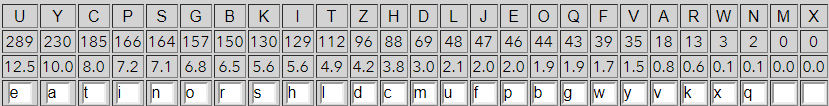
\includegraphics[width=\textwidth,height=\textheight,keepaspectratio]{39568ffdefe30f32bc60e606f4fe08fe.png}\ \\

\textbf{Did you crack it by hand, or did you use a tool?}\ \\
An online tool was used to determine the frequency of letters in the encoded message. The tool also allowed for the easy substitution of letters in the encrypted message.

\end{solution}

\end{document}
